\begin{center}
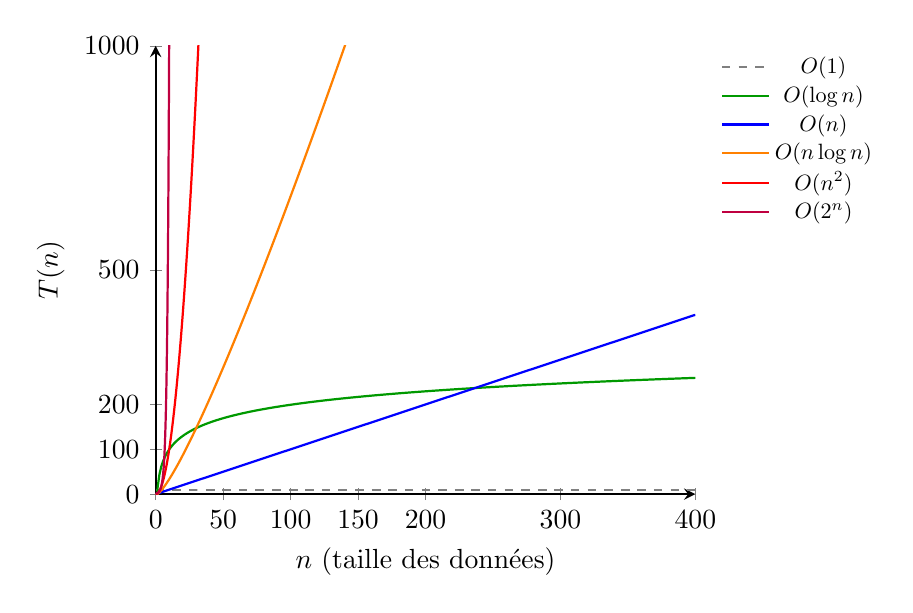
\begin{tikzpicture}[scale=1]
    \begin{axis}[
        axis lines = left,
        xlabel = {$n$ (taille des données)},
        ylabel = {$T(n)$},
        % n s'etend jusqu'a 200
        xmin=0, xmax=400,
        % Le plafond reste a 1000 pour forcer la sortie de cadre
        ymin=0, ymax=1000,
        % Graduation claire
        ytick={0, 100, 200, 500, 1000},
        yticklabels={0, 100, 200, 500, 1000},
        xtick={0, 50, 100, 150, 200, 300, 400},
        % Legende a droite a l'exterieur
        legend pos=outer north east,
        legend style={
            nodes={scale=0.8, transform shape},
            draw=none
        },
        domain=0.1:400,
        samples=300,
        thick,
        no markers
    ]
    % 1. O(1) - Constante
    \addplot [color=gray, dashed] {10}; 
    \addlegendentry{$O(1)$}
    
    % 2. O(log n) - Logarithmique
    \addplot [color=green!60!black] {30 * ln(x)/ln(2)}; 
    \addlegendentry{$O(\log n)$}
    
    % 3. O(n) - Lineaire
    \addplot [color=blue] {x}; 
    \addlegendentry{$O(n)$}
    
    % 4. O(n log n) - Quasi-lineaire
    \addplot [color=orange] {x*ln(x)/ln(2)}; 
    \addlegendentry{$O(n \log n)$}
    
    % 5. O(n^2) - Quadratique
    % Sort du cadre des n=32
    \addplot [color=red, domain=0:32] {x^2}; 
    \addlegendentry{$O(n^2)$}
    
    % 6. O(2^n) - Exponentielle
    % Sort du cadre immediatement (n=10)
    \addplot [color=purple, domain=0:10] {2^x}; 
    \addlegendentry{$O(2^n)$}
    
    \end{axis}
\end{tikzpicture}
\end{center}